\documentclass[11pt,a4paper]{colorart}

%%%%%%%%%%%%%%%%%%%%%%%%%%%%%%%%%%%%%%%%%%%%%%%%%%%%%%%%%%%%%%%%%%%%%%%%%%%%%%%%

\usepackage{graphicx}
\usepackage{amsmath}
\usepackage{bm}
\usepackage{latexsym}
\usepackage{amsfonts,amssymb}
\usepackage{psfrag}
\usepackage{ulem}
\usepackage{textcomp}
\usepackage{color}
\usepackage{physics}
\usepackage{amsthm}
\usepackage{mathrsfs}
\usepackage{tikz-cd}
\usepackage{listings}
\usepackage{xcolor}
\usepackage{hyperref}
%%%%%%%%%%%%%%%%%%%%%%%%%%%%%%%%%%%%%%%%%%%%%%%%%%%%%%%%%%%%%%%%%%%%%%%%%%%%%%%

\def\nn{\nonumber} 
\def\pa{{\partial}}
\def\f{\frac}
\def\l{\left}
\def\r{\right}
\def\d{{\rm d}}
\def\es{\emptyset}
\def\R{\mathbb{R}}
\def\C{\mathbb{C}}
\def\N{\mathbb{N}}
\def\Z{\mathbb{Z}}
\def\Q{\mathbb{Q}}
\def\e{\epsilon}
\def\a{\alpha}
\def\b{\beta}
\def\g{\gamma}
\def\p{\phi}
%%%%%%%%%%%%%%%%%%%%%%%%%%%%%%%%%%%%%%%%%%%%%%%%%%%%%%%%%%%%%%%%%%%%%%%%%%%%%%%

\numberwithin{equation}{section}
\makeatletter
\def\bign#1{\mathclose{\hbox{$\left#1\vbox to8.5\p@{}\right.\n@space$}}\mathopen{}} %define a good looking A/~ symbol
%\@addtoreset{section}{part} %comment this if not using parts
\makeatother
\allowdisplaybreaks
%\renewcommand*\thesection{\thepart.\arabic{section}} %comment this if not using parts
%------
%---tikz environment---
\usetikzlibrary{arrows}
%-------
%---hyperref (comment this if not using parts)---
%\renewcommand{\thehsection}{\thepart.section.\thesection}
%---------
%%%%%%%%%%%%%%%%%%%%%%%%%%%%%%%%%%%%%%%%%%%%%%%%%%%%%%%%%%%%%%%%%%%%%%%%%%%%%%%%
\definecolor{codegreen}{rgb}{0,0.6,0}
\definecolor{codegray}{rgb}{0.5,0.5,0.5}
\definecolor{codepurple}{rgb}{0.58,0,0.82}
\definecolor{backcolour}{rgb}{0.95,0.95,0.92}

\lstdefinestyle{mystyle}{
    backgroundcolor=\color{backcolour},   
    commentstyle=\color{codegreen},
    keywordstyle=\color{magenta},
    numberstyle=\tiny\color{codegray},
    stringstyle=\color{codepurple},
    basicstyle=\ttfamily\footnotesize,
    breakatwhitespace=false,         
    breaklines=true,                 
    captionpos=b,                    
    keepspaces=true,                 
    numbers=left,                    
    numbersep=5pt,                  
    showspaces=false,                
    showstringspaces=false,
    showtabs=false,                  
    tabsize=2
}

\lstset{style=mystyle}
%%%%%%%%%%%%%%%%%%%%%%%%%%%%%%%%%%%%%%%%%%%%%%%%%%%%%%%%%%%%%%%%%%%%%%%%%%%%%%%%

\begin{document}
%%%%%%%%%%%%%%%%%%%%%%%%%%%%%%%%%%%%%%%%%%%%%%%%%%%%%%%%%%%%%%%%%%%%%%%%%%%%%%%%
\title{\huge Congruent Numbers and Tunnell's theorem \footnote{All the source code used here has been uploaded on \href{https://github.com/ManuSomvanshi/ConguentNumber}{\textcolor{red}{github}}.}}
\author{Manvendra Somvanshi (MS20126)} 
\date{\today} 
%%%%%%%%%%%%%%%%%%%%%%%%%%%%%%%%%%%%%%%%%%%%%%%%%%%%%%%%%%%%%%%%%%%%%%%%%%%%%%%%
\maketitle
\tableofcontents
\vspace{5pt}
\hrule
\vspace{6pt}
\section{Congruent Numbers and the Problem}
The congruent number problem is ancient problem in number theory. A congruent number is defined as follows.
\begin{definition}
  An positive integer $n$ is said to be a congruent number if there exists a right angle triangle with rational sides such that $n$ is the area of that triangle. 
\end{definition}
The congruent number problem asks whether it is possible to devise a simple enough test to check if an integer is congruent. Here "simple enough" means that the congruency of the number can be determined in polynomial time. Using the concept of Pythagoras triplets it easy enough to generate right triangles. This technique can be used to generate all the congruent numbers as well. Let $a,b$ be two integers. Then $x = a^2-b^2, y = 2ab, z = a^2+b^2$ satisfies the condition $x^2+y^2 = z^2$. If $g$ is the g.c.d. of $a,b$ then $a = gc$ and $b = gd$ where $\gcd(c,d) = 1$. Let $x' = c^2 - d^2, y' = 2cd, z' = c^2+d^2$. Then we can have
\begin{align*}
  x = g^2x',\ y = g^2 y',\And z = g^2z'.
\end{align*}
Moreover when $c,d$ are both not odd together then $(x',y',z')$ are primitive Pythagoras triplets (i.e. they have no common divisor). Now consider the following result.
\begin{proposition}
  An integer $n$ is congruent if it's square free part is congruent.
\end{proposition}
\begin{proof}
  Consider an integer $n = s^2m$, where $m$ is square free. Then there exist $x,y,z\in \Q^*$ such that $z^2 = x^2 + y^2$ and $m = \f{1}{2}xy$. Then the number $n = s^2m$ corresponds to the area of the triangle with sides $sx, sy, sz$.
\end{proof}
This result leads to the following definition of an equivalence relation on $\Z^+$: let $x\sim y$ if either $x = s^2y$ or $y = s^2 x$ for some $s\in Z$. Let $S$ be the $\Z^+\bign/ \sim$. $S$ has an equivalence class for each square free integer. By the previous proposition it is enough to check congruence of elements in $S$. Returning back to the problem of generating congruent numbers: since the primitive Pythagoras triplets can generate any Pythagoras triplet with area of the respective triangles differing by factor of a square, it follows that looking at primitive Pythagoras triplets is enough. This discussion is summarised in the following theorem.
\begin{theorem}\label{thm:cong_gen}
  For every congruent number $n$ there exists integers $a,b$ such that $\gcd(a,b) = 1$, $a,b$ are both not odd, and $n \sim ab(a^2-b^2)$. 
\end{theorem}
\begin{proof}
  For $n$ there exists rationals $x,y,z$ such that $n = \f{1}{2}xy$ and $x^2 + y^2 = z^2$. Suppose that $x = p/q, y = r/s, z = t/u$ then $n' = \f{1}{2}(prqs)u^2 = n(q^2s^2u^2)$ is the area of the triangle with integer sides $psu, rqu, qst$. By definition $n\sim n'$. Since primitive Pythagoras triplets generates Pythagoras triplets it follows that there is some Pythagoras triplet $x',y',z'\in \Z^+$ such that they are coprime. Since every primitive Pythagoras triplet can be written as $x' = a^2 - b^2, y' = 2ab, z' = a^2 + b^2$ where $a,b$ are coprime and both are not odd, the conclusion follows.
\end{proof}
\begin{remark}
Using \cref{thm:cong_gen} it follows that every primitive Pythagoras triplet generate the set of squarefree congruent numbers. I have written a program (discussed later) which will generate a list of congruent numbers. But note that it is not possible to know a specific congruent number would appear in this list.
\end{remark}
\begin{proposition}\label{pro:rational_sq}
  An integer $n$ is congruent if and only if there exists $a\in \Q^+$ such that $a, a \pm n$ are rational squares.
\end{proposition}
\begin{proof}
  Suppose that $n$ is congruent. Then there exists rational $x,y,z$ such that $x^2 +y^2 =z^2$ and $n = \f{1}{2}xy$. Thus it follows that
  \begin{align}\label{eq:1.1}
    x^2 + y^2 \pm 4n &= z^2 \pm 4n \nonumber\\
    \implies (x\pm y)^2 &= z^2 \pm 4n \nonumber\\
    \implies \l(\f{x\pm y}{2}\r)^2 &= \l(\f{z}{2}\r)^2 \pm n
  \end{align}
  Thus we get $a = (z/2)^2$. Conversly suppose that there is an $a$ such that $a, a \pm n$ are a rational squares. Then let $x = \sqrt{a + n} - \sqrt{a - n}, y = \sqrt{a + n} + \sqrt{a -n}, z = 2\sqrt{a}$. Then we clearly have $x^2 + y^2 = z^2$ and $n = \f{1}{2}xy$.
\end{proof}

\begin{theorem}[Fermat]
  $1$ is not a congruent number.
\end{theorem}
\begin{proof}
  Suppose that $1$ is congruent. Then there exists an $a\in \Q^+$ such that $a\pm 1, a$ are rational squares. Suppose that $\sqrt{a} = \f{u}{v}$ such that $u,v$ are coprime. Then
  \begin{align*}
    a\pm 1 & = \f{u^2 \pm v^2}{v^2}
  \end{align*}
  Multiplying these we get that
  \begin{align*}
    v^4(a^2-1) = u^4 - v^4.
  \end{align*}
  Note that the LHS is a perfect integer square as well. Thus there exists an integral solution to the equation
  \begin{align*}
    X^4 - Y^4 = Z^2
  \end{align*}
  This is a contradiction since the above equation has no solutions.
\end{proof}

\begin{corollary}
  Perfect squares are not congruent.
\end{corollary}
\begin{proof}
  Since the square free part of perfect squares is $1$, it follows that $n$ is not congruent. 
\end{proof}
\begin{remark}
  The above corollary has an interesting geometric interpretation as well. Given any right angle triangle with rational sides and area $n\in \N$ it is not possible to construct a square of rational side with area $n$.
\end{remark}

\section{Elliptic Curves and Tunnell's Theorem}
Consider the \cref{eq:1.1} in \cref{pro:rational_sq}. We can multiply the two equations together to obtain
\begin{align*}
  \l(\f{x^2 - y^2}{4}\r)^2 &= \f{z^4}{16} - n^2
\end{align*}
Thus it follows that there exists a rational solution to the equation
\begin{align*}
  v^2 = u^4 - n^2
\end{align*}
where $v = (x^2 - y^2)/4, u = z/2$. Multiplying this equation by $u^2$ and setting $X = u^2$ and $Y = uv$ we get
\begin{align}\label{eq:elliptic}
  Y^2 = X^3 - n^2X
\end{align}
Thus given a right angle triangle which has rational sides and area $n$, there exists a point $(X,Y)\in \Q^2$ which lies on the curve given by \cref{eq:elliptic}. An interesting question to ask at this point is whether every rational point on this curve corresponds to a right triangle with rational sides and area $n$? This is not true in general since the $X$ coordinate must be a rational square (by the construction above). But a classification of such rational points on the curve \cref{eq:elliptic} is possible, as shown in the following theorem.

\begin{theorem}
  Let $(X,Y)$ be a rational point on the curve $Y^2 = X^3 - n^2X$ such that
  \begin{enumerate}
    \item $X$ is a rational square.
    \item $X$ has an even denominator.
  \end{enumerate}
  Then there exists a right angle triangle with rational sides and area $n$.
\end{theorem}
\begin{proof}
  Let $u = \sqrt{X}$ and $v = Y/u$. Then we get that
  \begin{align*}
    &v^2u^2 = u^6 - n^2 u^2\\
    \implies &v^2 = u^4 - n^2\\
    \implies &v^2 + n^2 = x^2
  \end{align*}
  Let $u = p/q$ where $p,q$ are coprime. Then by assumption $q$ is even. Since $n$ is an integer it follows that $v^2$ and $x^2$ have the same denominator, i.e. $q^4$. Clearly $q^2v, q^2n, q^2x$ is a primitive Pythagoras triplet. Thus there exists $a,b$ coprime and $a+b$ odd, such that $q^2v = a^2 - b^2, q^2n = 2ab$, and $q^2x = a^2 + b^2$. Then the right angle triangle with sides $x = 2a/q, y = 2b/q,$ and $z = 2u$ has area $n$.
\end{proof}

\begin{definition}
  Let $K$ be some field with characteristic $\neq 2$ and let $f\in K[x]$ be a cubic polynomial with distinct roots in some extension $K'$ of $K$. Then the set of solutions to the equation
  \begin{align*}
    E:\ y^2 = f(x),
  \end{align*}
  where $x,y$ are in $K'$, are called the $K'$ points of an elliptic curve. Represent this set by $E(K)$.
\end{definition}

Till now we had been working with the elliptic curve $y^2 = x^3 - n^2x$ over the field $K = K' =\Q$. This is an elliptic curve because the roots of the polynomial $x^3 - n^3x$ are $0, \pm n$ (distinct in $\Q$). Thus the congruent number problem is very closely related to the study of elliptic curves.\\

%\begin{definition}
%  Let $K$ be a field. Consider the following equivalence relation on $K^3$,
%  \begin{align*}
%    (x,y,z) \sim (x',y',z') \iff \exists \lambda\in K\ \text{s.t.}\ (x,y,z) = (\lambda x', \lambda y', \lambda z').
%  \end{align*}
%  Then the set $ \mathbb{P}^2_K \coloneqq K^3-\{(0,0,0)\}\bign/\sim$ is called the projective plane.
%\end{definition}

Consider an elliptic curve $E(K)$ over some field $K$. Define an addition on $E(K)$ in the following way: consider 2 $K-$points $P,Q$, on the elliptic curve $E(K)$. Draw a line joining $P,Q$. This would intersect the curve at a third point $R$. Then define $P+Q = -R$, where $-R = (a,-b)$ if $R=(a,b)$. Let $O$ be the (unique) point at infinity. This addition makes $E(K)$ an abelian group with identiy $O$. The inverse of a point is $P$ is just $-P$.

\begin{definition}
  If $G$ is a group then the subgroup containing all finite order elements is called the torsion subgroup $G_{\text{tors}}$ of $G$.
\end{definition}
\begin{theorem}[Mordell-Weil]
  If $E(\Q)$ is a an elliptic curve then it is finitely generated and $E(\Q) \cong E(Q)_{\text{tors}} \times \Z^r$.
\end{theorem}
Here the number $r$ is called the rank of the elliptic curve.
\begin{conjecture}[Birch and Swinnerton-Dyer (BSD)]
  Let $E$ be an elliptic curve and $x$ be some integer, then
  \begin{align*}
    \prod_{p\ |\ x} \f{\# E(\mathbb{F}_p)}{p} \sim C_E (\log(x))^{\text{rank}(E(\Q))}.
  \end{align*}
\end{conjecture}
Now we can finally understand the statement of the amazing theorem proved by Tunnell regarding to classify congruent numbers.
\begin{theorem}[Tunnell]
  Let $n$ be a square free positive integer. Then define the following:
  \begin{align*}
    a_n &= \#\{(x,y,z)\in \Z^3\ |\ 2x^2 +y^2+8z^2 = n\}\\
    b_n &= \#\{(x,y,z)\in \Z^3\ |\ 2x^2 +y^2+32z^2 = n\}\\
    a'_n &= \#\{(x,y,z)\in \Z^3\ |\ 8x^2 +2y^2+16z^2 = n\}\\
    b'_n &= \#\{(x,y,z)\in \Z^3\ |\ 8x^2 +2y^2+64z^2 = n\}.
  \end{align*}
  Then,
  \begin{enumerate}
    \item If $n$ is an odd congruent number then $a_n = 2b_n$. If $n$ is an even congruent number then $a'_n = 2b'_n$.
    \item The converse of statement 1 is true if the BSD conjecture is assumed.
  \end{enumerate}
\end{theorem}

An immidiate corollary to Tunnell's theorem is the following.
\begin{corollary}
  Let $n$ be an integer. $n$ is congruent if $n \equiv 5,6,7 \pmod{8}$.
\end{corollary}

\section{Computation of Congruent Numbers}
There are three essentially three computations which I have done.
\begin{enumerate}
  \item The first is brute force computation of congruent numbers using the Pythagoras triplet method discussed in \cref{thm:cong_gen}.
  \item The second is generating the congruent numbers assuming that the BSD conjecture (and hence the converse in Tunnell's theorem) holds true.
  \item The distribution of congruent numbers assuming the BSD conjecture.
\end{enumerate}
\subsection{Brute force Method}
In this method I first generate pairs $(a,b)$ such that $\gcd(a,b) = 1$ and $a+b$ is odd and for each pair the right angle triangle and its area is calculated and added to a list of dictionaries. This is done by the following snippet:
\lstinputlisting[language = Python, firstline = 8, lastline = 20]{code/check_cong.py}
To generate the list of square free congruent numbers I add the "area" key in the dictionary to a set, after removing the square part from the integer. 
\lstinputlisting[language = Python, firstline = 35, lastline = 42]{code/check_cong.py}
This method gives the following output when $N = 40$.
\lstinputlisting{code/bruteforce.txt}
As evident this method is very inefficient to generate congruent numbers. For example the number $13$, which is congruent, has not appeared in this list yet even after $40$ trials.

\subsection{Tunnell's method}
In this method we assume that the BSD conjecture is true and use the converse of Tunnell's theorem to generate a list by checking if each integer below some $N$ is congruent or not. This gives an exhaustive list congruent numbers below $N$. This is much better than the previous method which just gives us $N$ congruent numbers.
\lstinputlisting[language = Python, firstline = 44, lastline = 77]{code/check_cong.py}
Here are all the square free congruent numbers less than $1000$:
\lstinputlisting{code/tunnell.txt}

\subsection{Distribution of square free congruent numbers}
I wrote a method that counts the number of square free congruent numbers less than $N$ using Tunnell's method (assuming the BSD conjecture) and I have plotted their ratio against $N$.
\lstinputlisting[language = Python, firstline = 83, lastline = 92]{code/check_cong.py}
\begin{figure}
  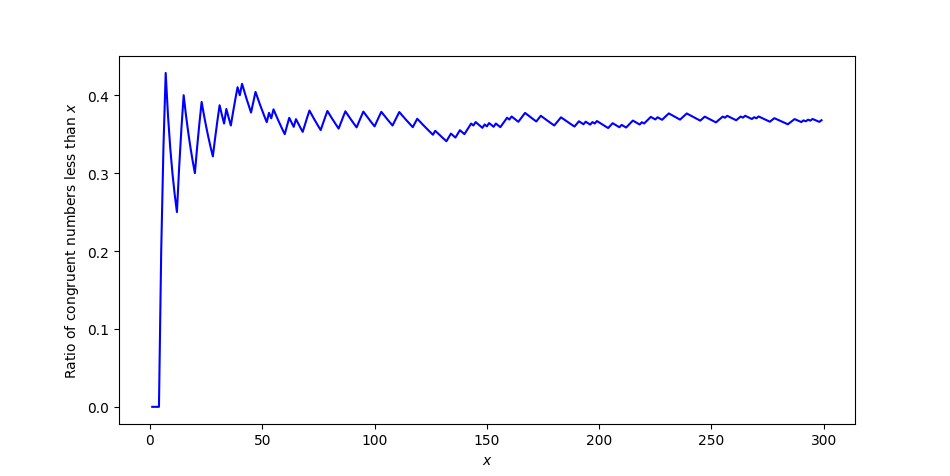
\includegraphics[width = \textwidth]{code/distribution2.png}
  \caption{The distribution for $N = 500$. As observed here this ratio eventually becomes a constant with value of about $0.368$.}
\end{figure}
From the above figure one can also claim the following conjecture.
\begin{conjecture}
  For large enough $n$ the number of square free congruent numbers, $C(n)$, less than $n$ can be approximated by
  \begin{align*}
    C(n) \sim \a n
  \end{align*}
  where $\a \approx 0.368$.
\end{conjecture}
This conjecture will be true given the assumption of the BSD conjecture.

\end{document}
